% !TEX root = thesis.tex

\chapter{Data analysis}
\label{cha:data_analysis}
The datasets created allow to perform some measurement regarding the use of scholarly works in the English Wikipedia.
\todo{TODO\@: other statistics? Maybe some that use the pagecounts?}

\section{Wikipedia articles}
\subsection{Where do identifiers appear in a Wikipedia article?}

\subsection{How many sections Wikipedia articles have?}

\subsection{Which are the most common sections in Wikipedia articles?}

\section{Papers in Wikipedia}
This section analyzes the use of papers in wikipedia.

\subsection{Incoming citations distribution}
The distribution of scholarly citations has been studied many times by the scientific community.
The problem is to discovery what is the distribution of citations, that is the number of papers cited a total number of $x$ times, $N(x)$.
Redner~\cite{Redner1998} suggested that this distribution has a large-$x$ power law decay $N(x) \sim x^{-\alpha}$.

Fig.~\ref{fig:incoming_citations_loglog} compares the distribution of citations of all the papers in history and the ones found only in Wikipedia.
The number of incoming citation for a paper is determined using the \ac{MAG} dataset.
Notice that because of the data available in the \ac{MAG}, only the papers found in Wikipedia which have a \ac{DOI} are considered.
This account for the 28\% of the identifiers found.
Furthermore, from this set of papers we removed the ones that appears to be ``non-valid'' in the \ac{MAG} dataset, namely the ones that have more than one \ac{DOI}.
The amount of papers considered at the end is 17\% of the identifiers found in wikipedia.

From the graph we can only see that both the distribution follow some kind of power law.
It is more interesting to analyze the \ac{CCDF} of the two series.
In our case, the \ac{CCDF}, or \emph{tail distribution}, expresses the percentage of papers $\bar{F}(x)$ that have more than $x$ citations.

From Fig.~\ref{fig:incoming_citations_ccdf_1000}~and~\ref{fig:incoming_citations_ccdf_100} we can see that papers appearing in Wikipedia tend to have many more incoming citations with respect to a random paper taken from all the available ones.
For instance, the 74\% of papers in Wikipedia have at least 10 incoming citations, while only the 13\% of papers have at least 10 incoming citations.
\todo{Regarding the ``All papers'' serie, should we limit only papers having DOIs?}
% see https://en.wikipedia.org/wiki/User:ProteinBoxBot.


\begin{figure}[h]
\centering
\includegraphics[keepaspectratio=true, width=\textwidth]{assets/incoming_cits_loglog}
\caption{Incoming citations distribution of papers appearing in the \emph{mag} datasets and the ones appearing only in English Wikipedia, on a log-log scale.}
\label{fig:incoming_citations_loglog}
\end{figure}

\begin{figure}[h]
\centering
\includegraphics[keepaspectratio=true, width=\textwidth]{assets/incoming_cits_ccdf_1000}
\caption{Complementary cumulative distribution function of the first 100 incoming citations of papers appearing in the \emph{mag} datasets and the ones appearing only in English Wikipedia.}
\label{fig:incoming_citations_ccdf_1000}
\end{figure}

\begin{figure}[h]
\centering
\includegraphics[keepaspectratio=true, width=\textwidth]{assets/incoming_cits_ccdf_100}
\caption{Complementary cumulative distribution function of the first 100 incoming citations of papers appearing in the \emph{mag} datasets and the ones appearing only in English Wikipedia.}
\label{fig:incoming_citations_ccdf_100}
\end{figure}

\subsection{Age of identifiers at first appearance}
During the analysis of the data we have obtained from Wikipedia, an interesting information came up: the age of the papers when they first appear in Wikipedia.
Fig.~\ref{fig:age_of_papers_at_first_appearance} shows the distribution of the age of papers when they are inserted on Wikipedia for the first time.
In theory there should not be negative values, because this would mean that an identifier appears in Wikipedia before the paper is published.
In practice this happens because the \ac{MAG} dataset is not 100\% accurate, and some publication dates may contain errors.
We have investigate this problem, and it seems to be caused by indexing engine used by Microsoft.
It seems that if a paper is published online on a certain date, and it is also released after in a journal, Microsoft consider the date of the journal the publication date.
However, only the 3,12\% of the \acp{DOI} extracted have a negative age.

It is interesting to see that many \acp{DOI} are inserted in Wikipedia few days after their publication (Fig.~\ref{fig:age_of_papers_at_first_appearance_zoom}).
A possible explanation is that some authors insert the identifier of their paper as soon as it has been published.

Finally, to give a scale to this numbers, Fig.~\ref{fig:age_of_papers_at_first_appearance_cdf} measure is the \ac{CDF} of the serie, namely what is the percentage $F(x)$ of paper identifiers inserted in Wikipedia at most $x$ days after their publication.
\todo{conclude, somehow}

% Notes:
% Kamil Crater (doi 10.1126/science.1190990) has been added by the author as soon as possible. \url{https://en.wikipedia.org/w/index.php?title=Kamil_Crater&diff=next&oldid=375884625}

\begin{figure}[h]
\centering
\includegraphics[keepaspectratio=true, width=\textwidth]{assets/age_of_papers_at_first_appearance}
\caption{Distribution of the age of papers when their DOI appear for the first time on Wikipedia.}
\label{fig:age_of_papers_at_first_appearance}
\end{figure}

\begin{figure}[h]
\centering
\includegraphics[keepaspectratio=true, width=\textwidth]{assets/age_of_papers_at_first_appearance_-30+30}
\caption{Distribution of the age of papers when their DOI appear for the first time on Wikipedia, showing only ages between $[-30, 30]$ days.}
\label{fig:age_of_papers_at_first_appearance_zoom}
\end{figure}

\begin{figure}[h]
\centering
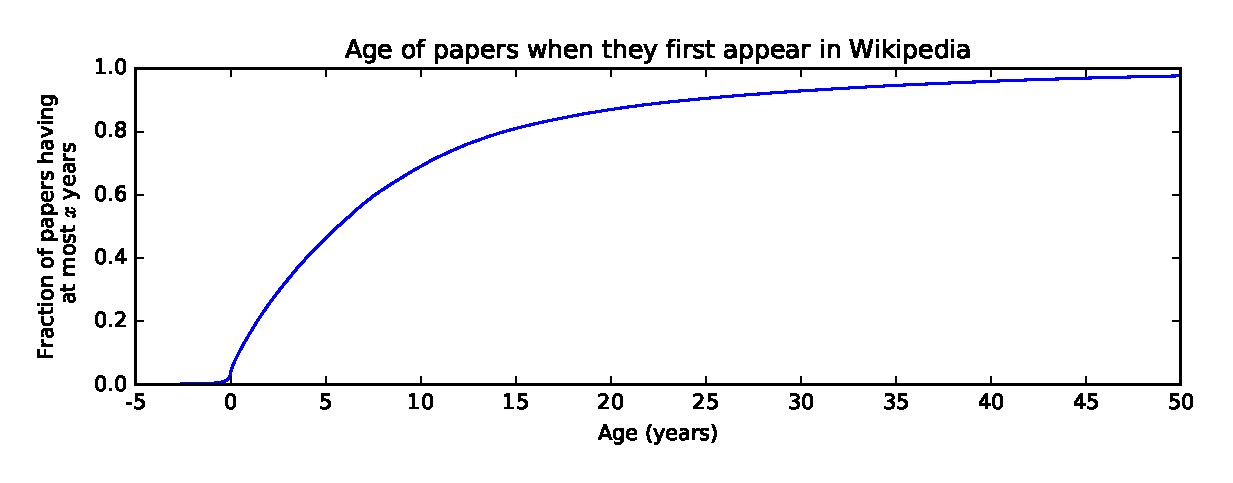
\includegraphics[keepaspectratio=true, width=\textwidth]{assets/age_of_papers_at_first_appearance_cdf}
\caption{todo}
\label{fig:age_of_papers_at_first_appearance_cdf}
\end{figure}

\subsection{Lifetime in a Wikipedia article}
todo: show graph of identifier insertions in time
analizza la persistenza degli identifier inseriti e rimossi

fare la average della persistenza degli identifier escludendo la coda
\subsection{Publication date distribution}
\subsection{Top cited journals by views}
